
\section{Performance-Analyse der vorgegebenen Python-Implementierung}

\subsection{Komplexität}
\begin{frame}{Komplexität}
	%TODO: unser Schiff soll schöner werden!
	\begin{center}
		$ R $ -- Anzahl der Pixel; $ R_{corr} $ -- Korrelationsgröße; $ n $ -- Anzahl der Bilder \\
	\end{center}
	\textbf{Hauptroutine:} \\
	\setlength\extrarowheight{5pt}
	\begin{center}
		\begin{tabular}{| >{\centering\arraybackslash}m{4cm} | >{\centering\arraybackslash}m{5cm} |}
			\hline
			Bild-Präprozessierschritte & $ \mathcal{O}(R) $ \\ \hline
			Speckle-Tracking & $\mathcal{O}\left(\frac{R \cdot R_{corr} \cdot log\left(R_{corr}\right) \cdot N_{corr}}{P_u^2 \cdot R_{grid}^2}\right) \approx \mathcal{O}\left(R \cdot R_{corr} \cdot log\left(R_{corr}\right)\right)$ \\ \hline
			Rekonstruktion der Wellenfront & $ \mathcal{O}(R * log(R)) $ \\ \hline
		\end{tabular}
	\end{center}
	\vspace{.5cm}
	\textbf{$ \Rightarrow $ Gesamtkomplexität:} $ \approx \mathcal{O}\left(n \cdot R \cdot R_{corr} \cdot log\left(R_{corr}\right)\right)$
\end{frame}

\subsection{Datensets}
\begin{frame}{Datensets}
	\textbf{Hauptroutine:}
	\begin{itemize}
		\item<3-> Experiment 6
		\begin{itemize}
			\item ROI Größe: 1450x1450 (Bild), 550x550 (Template)
			\item Gitterauflösung: 1
			\item Korrelationsgröße: 91
			\item unterschiedliche Pixelgröße
		\end{itemize}
		\item<4-> Lenses
		\begin{itemize}
			\item ROI Größe: 1450x1550 (Bild), 1450x1550 (Template)
			\item Gitterauflösung: 1
			\item Korrelationsgröße: 41
			\item gleiche Pixelgröße
		\end{itemize}
	\end{itemize}
\end{frame}

\subsection{Gesamtlaufzeit}
\begin{frame}[allowframebreaks]{Gesamtlaufzeit}
	%TODO: größer & besser lesbar
	\begin{center}
		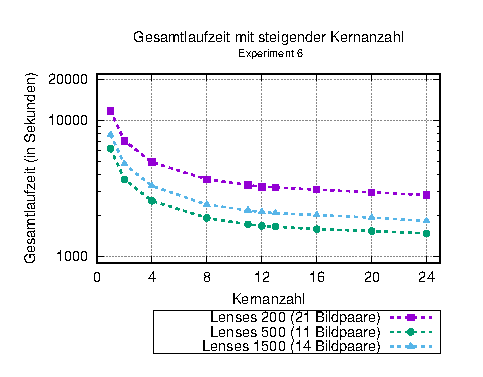
\includegraphics[width=0.6\linewidth]{pdf/times_exp6} \\
		\scriptsize
		Python 2.7, 2x Intel(R) Xeon(R) E5-2680 v3 (12 Kerne) @ 2.50GHz, kein MultiThreading
	\end{center}
	
	\framebreak
	
	\begin{center}
		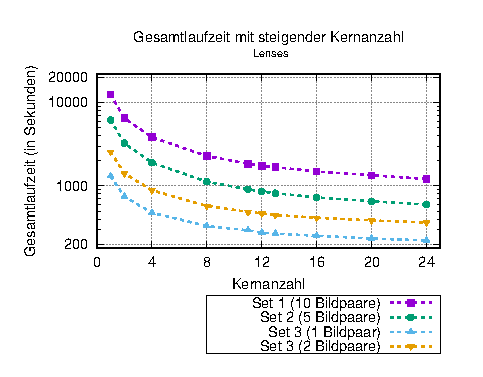
\includegraphics[width=0.6\linewidth]{pdf/times_lenses} \\
		\scriptsize
		Python 2.7, 2x Intel(R) Xeon(R) E5-2680 v3 (12 Kerne) @ 2.50GHz, kein MultiThreading
	\end{center}
\end{frame}

\subsection{Profiling}
\begin{frame}[allowframebreaks]{Profiling}
	\begin{center}
		%TODO: größer & besser lesbar
		\hspace{-0.7cm}
		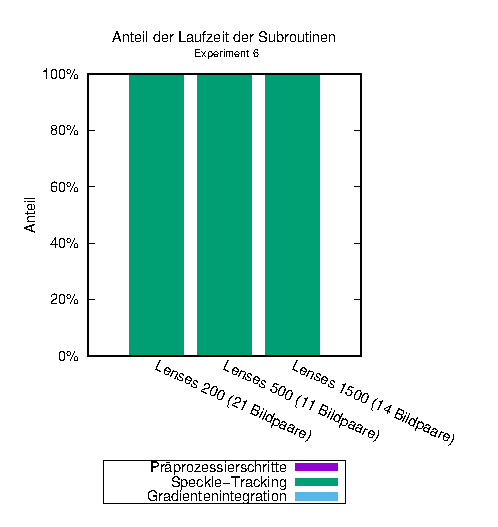
\includegraphics[width=0.4\linewidth]{pdf/main_exp6.eps}
		\hspace{-1.0cm}
		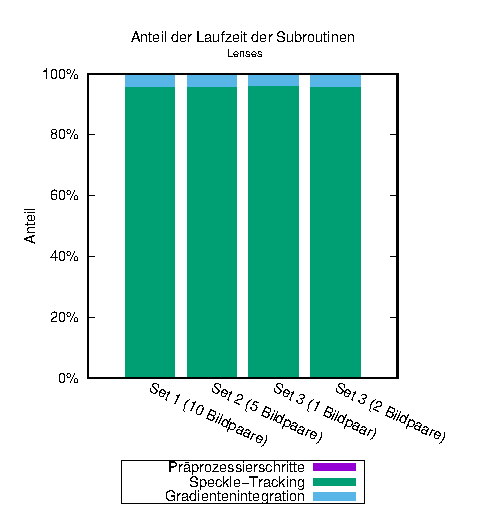
\includegraphics[width=0.4\linewidth]{pdf/main_lenses.eps}
		\hspace{-0.3cm}
		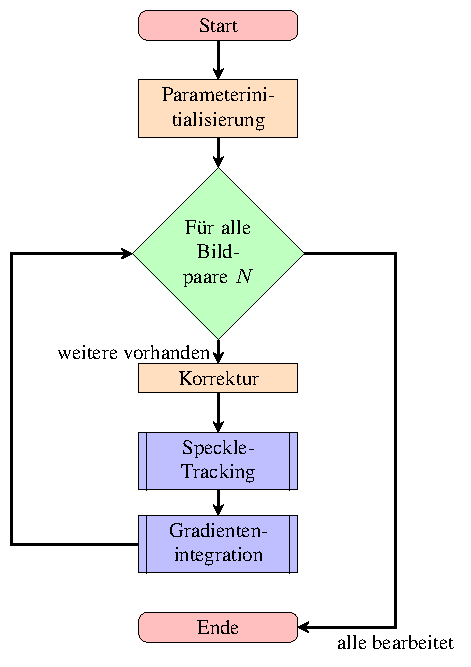
\includegraphics[width=0.33\linewidth]{pdf/graph_main}
		
		\framebreak
		
		\hspace{-0.9cm}
		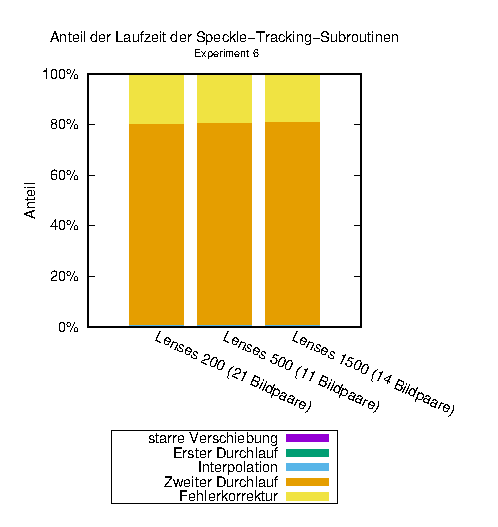
\includegraphics[width=0.47\linewidth]{pdf/speckle_exp6.eps}
		\hspace{-0.9cm}
		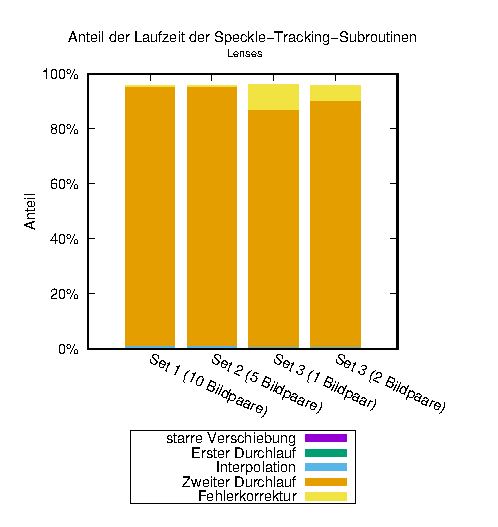
\includegraphics[width=0.47\linewidth]{pdf/speckle_lenses.eps}
		\hspace{-0.3cm}
		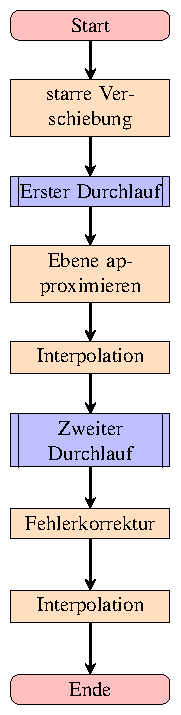
\includegraphics[width=0.15\linewidth]{pdf/graph_speckle}
		
		\framebreak
		
		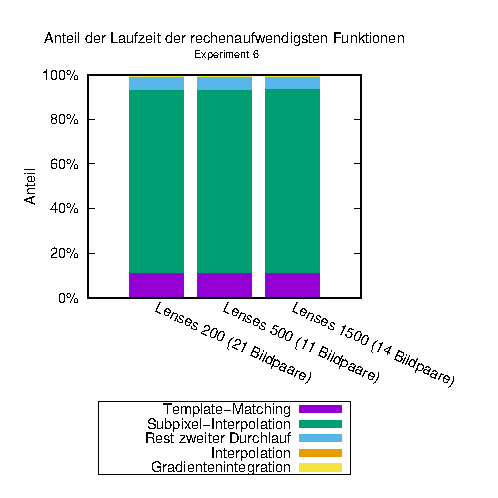
\includegraphics[width=0.53\linewidth]{pdf/slow_exp6.eps}
		\hspace{-1.5cm}
		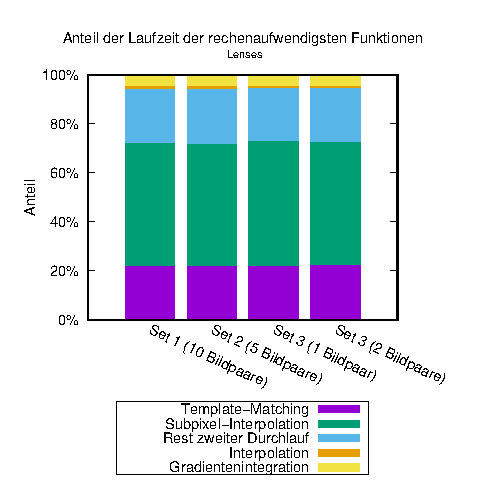
\includegraphics[width=0.53\linewidth]{pdf/slow_lenses.eps}\\
		\textbf{$ \Rightarrow $ über 95\%}
	\end{center}
\end{frame}
